\scanpage{74}
\mspage{73}
% E: drawing|top left|oriented rives and crossed coloured strands
\figure{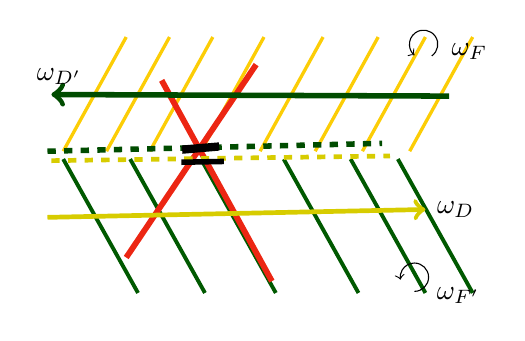
\begin{tikzpicture}[x=1cm,y=1cm]
\foreach \x in {-2.4,-1.85,-1.3,-.65,.1,.8,1.4,2}{\draw[yellow!65!orange,line width=1.2pt](\x,.1)--(\x+.8,1.55);}
\foreach \x in {-2.4,-1.55,-.65,.4,1.25,1.85}{\draw[green!35!black,line width=1.4pt](\x,0)--(\x+.95,-1.7);}
\draw[red!70!brown,line width=2.1pt](-1.15,1)--(.25,-1.55);\draw[red!70!brown,line width=2.1pt](.05,1.2)--(-1.6,-1.25);
\draw[green!30!black,line width=2pt,<-](-2.55,.82)--(2.5,.8);\node at(-2.45,1.05){$\omega_{D'}$};
\draw[yellow!65!olive,line width=1.7pt,->](-2.6,-.74)--(2.2,-.64) node[right,black]{$\omega_D$};
\draw[green!30!black,dashed,line width=2pt](-2.6,.1)--(1.65,.2);\draw[yellow!65!olive,dashed,line width=1.7pt](-2.55,-.02)--(1.75,.04);
\draw[line width=3pt](-.89,.12)--(-.42,.16);\draw[line width=2pt](-.9,-.04)--(-.36,-.03);
\draw[->](2.28,1.31)arc(-55:230:.18);\node at(2.76,1.37){$\omega_F$};
\draw[->](2.06,-1.68)arc(-90:190:.18);\node at(2.62,-1.73){$\omega_{F'}$};
\end{tikzpicture}}
% E: drawing|upper middle|alternative a' b' and reversed hatching
\figure{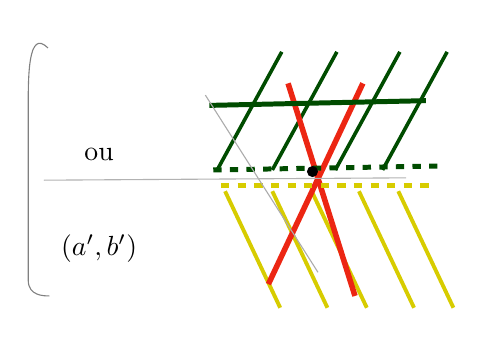
\begin{tikzpicture}[x=1cm,y=1cm]
\draw[gray](-2.45,1.55)..controls(-2.7,1.8)and(-2.7,1.2)..(-2.7,.8)--(-2.7,-1.4)..controls(-2.7,-1.6)and(-2.5,-1.6)..(-2.43,-1.6);
\node at(-1.8,.2){ou};\node at(-1.8,-1){$(a',b')$};
\foreach \x in {-.3,.4,1.2,1.8}{\draw[green!30!black,line width=1.3pt](\x,0)--(\x+.82,1.5);}
\foreach \x in {-.2,.4,.9,1.5,2}{\draw[yellow!65!olive,line width=1.4pt](\x,-.27)--(\x+.7,-1.75);}
\draw[red!70!brown,line width=2pt](.6,1.1)--(1.45,-1.6);\draw[red!70!brown,line width=2pt](1.55,1.1)--(.35,-1.45);
\draw[green!30!black,line width=1.8pt](-.4,.82)--(2.35,.88);
\draw[green!30!black,dashed,line width=1.8pt](-.35,0)--(2.5,.05);\draw[yellow!65!olive,dashed,line width=1.6pt](-.25,-.2)--(2.42,-.2);\fill(.91,-.02)circle(2pt);
\draw[gray!65](-.45,.95)--(.98,-1.3);\draw[gray!60](-2.5,-.13)--(2.1,-.1);
\end{tikzpicture}}
% E: text|upper right|car un peu vicieux
(car un peu vicieux, et sans intérêt!)
% E: text|left below figures|Cas a b de prolongation des rives
\deleted{\unsure{4)}} Cas $(a,b)$ \deleted{c'est le cas} de \uline{prolongation des rives}.
% E: text|left middle|1 On choisit comme recollement
1) On choisit comme recollement le transport parallèle. On trouve un $\mathcal X$ \deleted{avec} $\varphi:\mathcal X\longrightarrow X$ qui est une immersion.

Dans $\mathcal X$, on a un graphe \unsure{top.} $K$, et les faces de $(\mathcal X,K)$ correspondent aux p.r. stables \unsure{\&} \deleted{\unsure{on a un}} On a un $L=\varphi^{-1}(X_1)$, qui matérialise la corr. entre faces et p.r. stables --- en prolongeant chaque face $F$ par la face $\widetilde F$ obtenue en la ``renflant'' aux pts \deleted{qui} ``critiques'' de $S_K$ i.e. les pts de $K\cap S(L)$.
% E: text|right middle|NB Ici en partant d'une orientation
\uline{NB} Ici, en partant d'une orientation $\omega_F$ de $F=\Delta_D^*$, c.à.d. $\omega_D$ orientation de $D$, passant à l'orientation $\omega'$ de $\Delta_{D'}^*$ déduite par transport via le recollement, et \unsure{une} orientation $\omega_{D'}$ de $D'$, on constate encore que c'est l'\uline{opposée} de celle obtenue par transport parallèle!
% E: margin note|beside NB|D in Delta and D' in Delta'
\margin{\diagram{\begin{tikzcd}[row sep=small]
\unsure{D\subset\Delta_D^*|D_i\Delta_D^*}\arrow[d,bend left=30,"\text{pour}"]\\
D'\subset\Delta_{D'}^*
\end{tikzcd}}}
% E: margin note|right margin at opposite orientation|L'ennui c'est que
\margin{L'ennui, c'est que les circuits sont \unsure{stériles|triviaux}. On n'obtient \unsure{rien} par les bons circuits supersinguliers!}
% E: text|bottom right|2 Recollement par l'iso opposé
2) Recollement par l'iso. \inserted{$a\simeq b$} opposé au transport parallèle. Cette fois, c'est au niveau de la transition $\underline\omega_F\mathbin{-}\underline\omega_{F'}$, interprétée comme $\underline\omega_D\mathbin{-}\underline\omega_{D'}$, qu'on obtient le transport parallèle. Contrairement à ce que je croyais \inserted{\unsure{avoir vu}} on trouve les bons circuits autour des positions supersingulières
